\documentclass{article}
% LaTex packages 
\usepackage[utf8]{inputenc}
\usepackage{amsfonts}
\usepackage{amsmath}
\usepackage{amsthm}
\usepackage{tabto}
\usepackage{booktabs}
\usepackage{hyperref}
\usepackage{xspace}
\usepackage[utf8]{inputenc}
\usepackage{fancyvrb}
\usepackage{stmaryrd}
\usepackage{graphicx}
\usepackage{url}
\usepackage[onehalfspacing]{setspace}
% Theorems
\usepackage{pgf}
\usepackage{tikz}
\usetikzlibrary{arrows}
\usepackage{graphicx}
\usepackage{setspace}
\usepackage{amssymb}
\usepackage{mathtools}
\usepackage{tabto}
\usepackage[T1]{fontenc}
%\usepackage[a4paper,left=2cm,right=2cm,top=2cm,bottom=3cm]{geometry}
\usepackage{geometry}
 \geometry{
 a4paper,
 %total={170mm,257mm},
 %left=20mm,
 top=30mm,
 }

\newtheorem{thm}{Theorem}[section]
\newtheorem{cor}[thm]{Corollary}
\newtheorem{lem}[thm]{Lemma}
\newtheorem{prop}[thm]{Proposition}
\theoremstyle{definition}
\newtheorem{defn}[thm]{Definition}
\theoremstyle{remark}
\newtheorem{rem}[thm]{Remark}
\DeclarePairedDelimiter\ceil{\lceil}{\rceil}
\DeclarePairedDelimiter\floor{\lfloor}{\rfloor}
\newcommand{\eg}{e.g.,\xspace}
\newcommand{\encrypt}[1]{\ensuremath{E(#1)}\xspace}
\newcommand{\decrypt}[1]{\ensuremath{D(#1)}\xspace}

\renewcommand{\labelitemi}{$\bullet$}
\renewcommand{\labelitemii}{$\circ$}
\renewcommand{\labelitemiii}{$\cdot$}
\renewcommand{\labelitemiv}{$\ast$}

\usepackage{wrapfig}
\usepackage[font=small,labelfont=bf]{caption}

% ---- Bibliography ----

\usepackage{biblatex}
\addbibresource{references.bib}
%------------------------------------
\begin{document}
\title{Summary}
\author{\vspace{-2.0cm} Nicola Libera}
\date{May 2020}
\maketitle

\section{Introduction}
\begin{itemize}
    \item First usage of the term ‚Gamification‘ occurred in 2003 \cite{gamification}
    \item Until 2010 Gamification was only used in advertisement and marketing contexts \cite{gamification}
    \item Gamification = ''use of game design elements in non-game contexts'' \cite{gamification}
    \item The goal hereby is to make often boring tasks more interesting or even entertaining
    \item Boosts the motivation and concentration 
    \item Today it is used in a wide range of applications e.g. education and modern research
    \item Especially computer scientists are interested in the possibilities of gamification to gain data 
    \item In the time of the digitalization are still a lot of tasks that require human computation
    \item This means that a human has to annotate a data set to improve a system or to create a data set that can be used to train an algorithm (just an example)
    \item Gamification can help to collect a lot of data from different people with comparatively low costs
    \item Is a great chance for the field of Information Retrieval
    \item Needs some special characteristics to be fun and appealing – the so-called game mechanics and game elements
\end{itemize}

\section{Game Mechanics and Elements}
\begin{itemize}
    \item A wide range of characteristics that a game can have
    \item A combination of the single characteristics is possible in any way imaginable
    \item An analysis of games and research have lead to a collection of design elements
    \item A list of known game mechanics and -elements:
    \begin{itemize}
        \item ''\textbf{Rules} They define the admissible actions and the components of the game with which a player can interact.
        \item \textbf{Conflicts} Conflicts are a set of actions that have to be performed to reach a particular goal in the application but require efforts to be solved.
        \item \textbf{Rewards} Rewards represent the benefits obtained for having performed an action or solved a particular conflict.
        \item \textbf{Winning Conditions} Winning Conditions are the objectives that can be reached by overcoming particular conflicts.
        \item \textbf{Player Interactions} They regard the structure of interaction between a player, the system and any other possible player in the game, if present. The most common forms are cooperative, competitive or single player games.
        \item \textbf{Resources} They are assets owned by a player and used to accomplish a particular goal or collected to boast her prestige.
        \item \textbf{Feedback} It is used to inform the player about how well he is performing in the platform.
        \item \textbf{Capture} to take or destroy opponents’ resources, while avoiding the same occurrence on herself.
        \item \textbf{Chase} to catch an opponent or elude one, if you are the player being chased.
        \item \textbf{Rescue/Escape} to get a defined resource to safety.
        \item \textbf{Race} being the first to achieve a specific result.
        \item \textbf{Pattern} Building requires players to place resources in specific patterns, based on adjacent resources or resources in the same group/cluster, taking into consideration nonspatial properties like color, set completion, cluster size, occurrence in time, etc.
        \item \textbf{Memory} requires players to recall previous game events or information in order to reach an objective.
        \item \textbf{Action} programming every player must secretly choose the next ’n’ turns, and then each player plays their turns out according to the choices made.
        \item \textbf{Guessing/Betting} encourage or require players to predict certain outcomes within the game, eventually by betting money (real or in-game).
        \item \textbf{Consensus} requires the players to agree on a certain topic or outcome.
        \item \textbf{Drawing} requires sketching objects, marking areas or drawing lines in one way or another.'' \cite{information_retrieval}
    \end{itemize}
    
    \item Gamification
    \begin{itemize}
        \item ''\textbf{Points} numerical values that represent a measure of the skill of a player or expendable resources at her disposal.
        \item \textbf{Leaderboards} ordered list of players based on the points they have obtained in a specific game or system.
        \item \textbf{Achievements \& Badges} set of designer defined tasks used to guide the users towards a certain goal and track their progress in a system.
        \item \textbf{Collection \& Virtual Goods} game assets with perceived or real monetary value.
        \item \textbf{Unlockable} Features Benefits or special characteristics of the system that can be accessed just by the most valuable players.
        \item \textbf{Status \& Fame} Obtaining social endorsement based on the results obtained within the system.
        \item \textbf{Customization} possibility to modify the interface or hidden set'' \cite{information_retrieval}
    \end{itemize}

    \item Additional Elements: 
    \begin{itemize}
        \item ''Performance Graphs
        \item Meaningful Stories
        \item Avatars'' \cite{wiki}
        \item Challenge 
    \end{itemize}
    \item These points/elements are important to make the task/the game fun
    \item Another important part that is important for a game is the fact that it has to be played voluntarily
\end{itemize}

\section{State of the Art/Games}
\begin{itemize}
    \item  I found mainly 3 tasks for which games were developed when it comes to Gamification in Information Retrieval: 
    \begin{itemize}
        \item Labeling images, videos, and music
        \item Examine search behavior of users
        \item Research ‚findability‘ or retrievability of specific web pages using different search engines (improving search engines)
    \end{itemize}
    \item 3 research questions: 
    \begin{itemize}
        \item ''Games have to be (by definition) fun to play and so in turn, we need to ask: Can this be made a fun game?
        \item Is the data we get from Page Hunt comparable to data we get from other sources? Does the nature of the game change the data?
        \item Finally, how do we get useful data from this? Can we define a process that extracts useful information from the data?'' \cite{search_engines}
    \end{itemize}
    \item List and descriptions of some games:
    \begin{itemize}
        \item \textbf{PageHunt}: \cite{search_engines}
        \begin{itemize}
            \item Goal: Improving search engines, develop labels for web pages
            \item Single player
            \item The user is shown a web page that he/she has to find using a search engine
            \item Data that was collected: Web page id, queries that were tried, the rank of the page if the page was found, the points that were scored by the query, the time the user spend finding the page
            \item Has some functions to prevent frustration and inappropriate content
            \item Functionality to review queries so that the search behavior can be improved
            \item Functionality to prevent users from making too long queries (making sure that users make queries as they would normally do)
        \end{itemize}
        \item \textbf{PageRace}: \cite{search_engines}
        \begin{itemize}
            \item Competitive version of PageHunt
            \item 2 users playing against each other – who finds the web page first?
            \item Each player can see the last query and results of the opponent – to prevent duplication and to help the players making better queries
        \end{itemize}
        \item \textbf{PageMatch}: \cite{search_engines}
        \begin{itemize}
            \item Collaborative version of PageHunt
            \item 2 player play together
            \item They are shown a web page and have to enter queries for this page
            \item They win if they can guess correctly whether they see the same page or not
        \end{itemize}
        \item \textbf{PageFetch (2)}: \cite{pagefetch, pagefetch2}
        \begin{itemize}
            \item The same as PageHunt but suitable for children / developed for children
            \item Design more appealing for children
            \item Web pages divided into different topics that can be chosen from
            \item Goal: Research how children perform in search tasks
        \end{itemize}
        \item \textbf{Fu-Finder}: \cite{fufinder}
        \begin{itemize}
            \item Goal: Research search performance of different users, collecting data about the search-fu of users
            \item Search-fu = ''denotes the skill of user‘s search abilities'' \cite{fufinder}
        \end{itemize}
    \end{itemize}
    \item Research results from the games (especially the Page games): \cite{search_engines}
    \begin{itemize}
        \item Length of the URL plays a role in the retrievability of web pages
        \item Search performance of users was simulated realistic
        \item Provides ideas on how to improve search engines
    \end{itemize}
\end{itemize}


\section{Research without specific games}
\begin{itemize} 
    \item Comparison of meaning and points \cite{disassembling_gamification}
    \begin{itemize}
        \item Set up: Creating tags for images
        \item 4 user groups: 
        \begin{itemize}
            \item Meaning and no points,
            \item Meaning and points,
            \item No meaning and no points,
            \item No meaning and points
        \end{itemize}
        \item Meaning e.g. means locating/tagging images with tumors in them
        \item Study goal: Comparing the performance, time spend per tag, tag quality and intrinsic motivation of the different groups
        \item Results:
        \begin{itemize}
            \item ''participants perceived the task as significantly more valuable [...] and tended to perceive it as personally more important [...] when a meaningful frame was given, regardless of points'' \cite{disassembling_gamification}
            \item Tagging performance\\
            Overall more tags were create when points were involved, independent from provided meaning. Meaning itself did not affect the performance of users. (see Figure \ref{fig:2})
            \item Time spend per tag\\
            In this case meaning increased the time users spend an generating task and the addition of points increaded the time even more. (see Figure \ref{fig:3})
            \begin{figure}[ht!]
                \centering
                \begin{minipage}[b]{0.49\textwidth}
                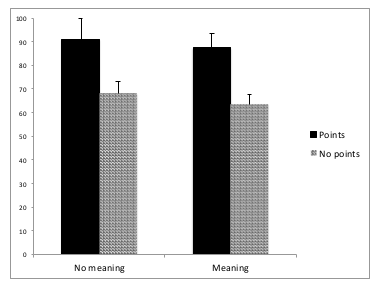
\includegraphics[width=1\textwidth]{images/Figure2_gamification.png}
                \caption{Average amount of tags per participant \cite{disassembling_gamification}}
                \label{fig:2}
                \end{minipage}
                \hfill
                \begin{minipage}[b]{0.5\textwidth}
                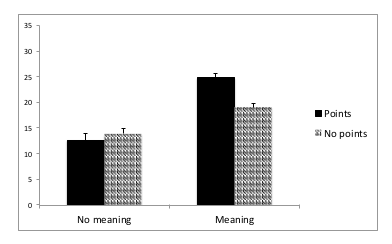
\includegraphics[width=1\textwidth]{images/Figure3_gamification.png}
                \caption{Average time spent per tag in seconds \cite{disassembling_gamification}}
                \label{fig:3}
                 \end{minipage}
            \end{figure}
            \item Quality\\
            A meaningful task resulted in higher quality, whereas points did not affect it significantly. (see Figure \ref{fig:4})
            \item Intrinsic motivation\\
            Meaning as well as only points increased the intrinsic motivation. In the groups with a meaningful task the addition or absence of points did not make a difference. (see Figure \ref{fig:6})
            \begin{figure}[ht!]
                \centering
                \begin{minipage}[b]{0.5\textwidth}
                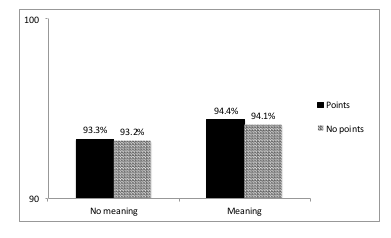
\includegraphics[width=1\textwidth]{images/Figure4_gamification.png}
                \caption{Quality tags in \% \cite{disassembling_gamification}}
                \label{fig:4} 
                \end{minipage}
                %\hfill
                \begin{minipage}[b]{0.49\textwidth}
                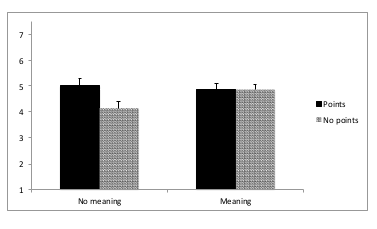
\includegraphics[width=1\textwidth]{images/Figure6_gamification.png}
                \caption{Mean intrinsic motivation \cite{disassembling_gamification}}
                \label{fig:6}
                 \end{minipage}
            \end{figure}
        \end{itemize}
    \end{itemize}
    
    
    \item How do users browse? \cite{user_behavior}
    \begin{itemize}
        \item Task: Finding 10 relevant documents within 50 clicks
        \item 2 versions: One just plain with a search bar, the corresponding results and the received points. The second with facets to choose from
        \item Results:
        \begin{itemize}
            \item Among other things, facets were found to increase the performance of users but are not necessarily considered as fun
        \end{itemize}
    \end{itemize}
    \item Comparison of points, leaderboards and levels \cite{game_elements}
    \begin{itemize}
        \item Task: Creating tags for images
        \item Research: Performance, intrinsic motivation, perceived autonomy and competence 
        \item Results:
        \begin{itemize}
            \item ''Implementation of these game elements significantly increased performance but did not affect perceived autonomy, competence or intrinsic motivation.'' \cite{game_elements}
            \item ''Cheating'' (nonsensical tags): levels(4.9\%), leaderboards (6.2\%), points (7.4\%), control group (8.2\%)
            \item Performance (number of created tags): control group < points < leaderboard $\approx$ levels
            \item Performance decreased in all groups over time but ''participants' performance in the leaderboard and levels conditions declined more slowly than in the other 2 conditions''\cite{game_elements} (see Figure \ref{fig:game_elements})
            \item Users provided with game elements generated more tags in the same amount of time as the control group
            \begin{figure}[h!]
                \centering
                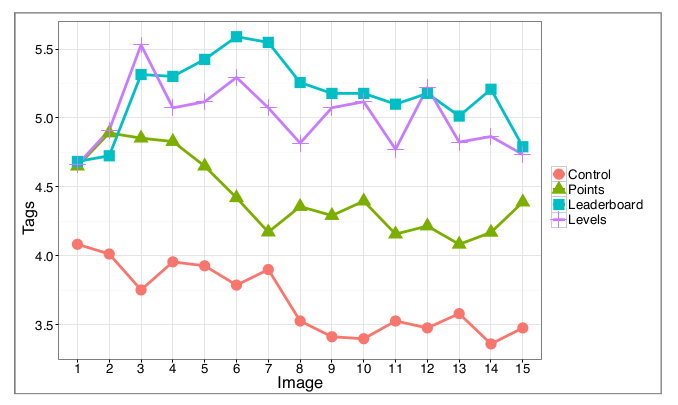
\includegraphics[width=0.7\textwidth]{images/game_elements.png}
                \caption{Average number of user-generated tags per condition over the course of 15 images. \cite{game_elements}}
                \label{fig:game_elements}
            \end{figure} 
        \end{itemize}
    \end{itemize}
\end{itemize}

\newpage

\section{Issues Regarding Gamification}
\begin{itemize}
    \item Making sure that the set up does not affect the natural behavior of the users in any way
\end{itemize}

\section{Used Software/Languages}
\begin{itemize}
    \item PageHunt: Microsoft Silverlight \cite{search_engines}
    \item PageFetch (2) \cite{pagefetch, pagefetch2}, Fu-Finder \cite{fufinder}: Python, Django, HTML, CSS, JavaScript
    \item PythonAnywhere for hosting the game
\end{itemize}

\section{Platforms}
Potential platforms to receive feedback for game:
\begin{itemize}
    \item Facebook
    \item itch.io
\end{itemize}

\section{Conclusion}
\begin{itemize}
    \item Very simple design in all applications - some are a bit more developed
    \item A lot of research concerning  the ''findability'' problem and search behavior
\end{itemize}


\section{Futre Work}
\begin{itemize}
    \item For the ''Page'' games: Usage of eye-tracking to see where users get useful information about the page for their query (can only be performed in a lab)
    \item Cursor movements could be an alternative for expensive and time consuming \cite{clicks}
\end{itemize}


\printbibliography
\end{document}
